\begin{figure}
\centering

\begin{subfigure}[b]{0.32\columnwidth}
\centering
\cfbox{box-gray}{
\resizebox{!}{\textwidth}{
\tikzsetnextfilename{inter2_1}
\begin{tikzpicture}[
mynode/.style={draw, circle, very thick, inner sep=1pt, scale=1.3},
myline/.style={draw, very thick},
]
\pgfmathsetmacro{\n}{14};
\pgfmathsetmacro{\r}{3};

\node[mynode,draw=Purple, circle] (1) at (0*360/\n + 90: \r cm)  {$\xcolor{P}_1^1$};
\node[mynode,draw=red] (2) at (1*360/\n + 90: \r cm)  {$\xcolor{R}_1^1$};
\node[mynode,draw=red] (3) at (2*360/\n + 90: \r cm)  {$\xcolor{R}_2^1$};
\node[mynode,draw=ForestGreen] (4) at (3*360/\n + 90: \r cm)  {$\xcolor{G}_1^1$};
\node[mynode,draw=ForestGreen] (5) at (4*360/\n + 90: \r cm)  {$\xcolor{G}_1^2$};
\node[mynode,draw=ForestGreen] (6) at (5*360/\n + 90: \r cm)  {$\xcolor{G}_2^1$};
\node[mynode,draw=ForestGreen] (7) at (6*360/\n + 90: \r cm)  {$\xcolor{G}_2^2$};
\node[mynode,draw=blue] (8) at (7*360/\n + 90: \r cm)  {$\xcolor{B}_1^1$};
\node[mynode,draw=blue] (9) at (8*360/\n + 90: \r cm)  {$\xcolor{B}_1^2$};
\node[mynode,draw=blue] (10) at (9*360/\n + 90: \r cm)  {$\xcolor{B}_1^3$};
\node[mynode,draw=YellowOrange] (11) at (10*360/\n + 90: \r cm)  {$\xcolor{O}_1^1$};
\node[mynode,draw=YellowOrange] (12) at (11*360/\n + 90: \r cm)  {$\xcolor{O}_1^2$};
\node[mynode,draw=YellowOrange] (13) at (12*360/\n + 90: \r cm)  {$\xcolor{O}_1^3$};
\node[mynode,draw=YellowOrange] (14) at (13*360/\n + 90: \r cm)  {$\xcolor{O}_1^4$};


\foreach \i in {1,...,\n}{
	\foreach \j in {\i,...,\n}{
    	\draw [myline,light-gray] (\i) -- (\j);
} }

\end{tikzpicture}
}
}
% \caption{All connections possible.\label{fig:inter2_1}}
\caption{$K_{14}$.\label{fig:inter2_1}}
\end{subfigure}
%
% \hspace{0.02\textwidth}
%
\begin{subfigure}[b]{0.32\columnwidth}
\centering
\cfbox{box-gray}{
\resizebox{!}{\textwidth}{
\tikzsetnextfilename{inter2_2}
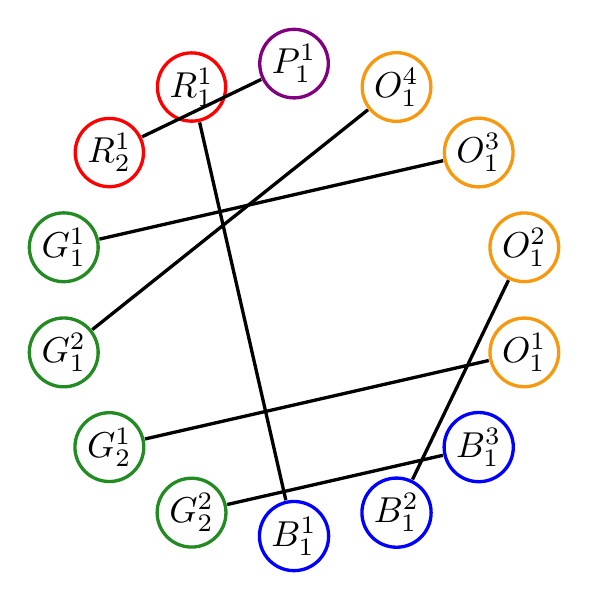
\begin{tikzpicture}[
mynode/.style={draw, circle, very thick, inner sep=1pt, scale=1.3},
myline/.style={draw, very thick},
]
\pgfmathsetmacro{\n}{14};
\pgfmathsetmacro{\r}{3};

\node[mynode,draw=Purple, circle] (1) at (0*360/\n + 90: \r cm)  {$\xcolor{P}_1^1$};
\node[mynode,draw=red] (2) at (1*360/\n + 90: \r cm)  {$\xcolor{R}_1^1$};
\node[mynode,draw=red] (3) at (2*360/\n + 90: \r cm)  {$\xcolor{R}_2^1$};
\node[mynode,draw=ForestGreen] (4) at (3*360/\n + 90: \r cm)  {$\xcolor{G}_1^1$};
\node[mynode,draw=ForestGreen] (5) at (4*360/\n + 90: \r cm)  {$\xcolor{G}_1^2$};
\node[mynode,draw=ForestGreen] (6) at (5*360/\n + 90: \r cm)  {$\xcolor{G}_2^1$};
\node[mynode,draw=ForestGreen] (7) at (6*360/\n + 90: \r cm)  {$\xcolor{G}_2^2$};
\node[mynode,draw=blue] (8) at (7*360/\n + 90: \r cm)  {$\xcolor{B}_1^1$};
\node[mynode,draw=blue] (9) at (8*360/\n + 90: \r cm)  {$\xcolor{B}_1^2$};
\node[mynode,draw=blue] (10) at (9*360/\n + 90: \r cm)  {$\xcolor{B}_1^3$};
\node[mynode,draw=YellowOrange] (11) at (10*360/\n + 90: \r cm)  {$\xcolor{O}_1^1$};
\node[mynode,draw=YellowOrange] (12) at (11*360/\n + 90: \r cm)  {$\xcolor{O}_1^2$};
\node[mynode,draw=YellowOrange] (13) at (12*360/\n + 90: \r cm)  {$\xcolor{O}_1^3$};
\node[mynode,draw=YellowOrange] (14) at (13*360/\n + 90: \r cm)  {$\xcolor{O}_1^4$};

\draw [myline] (14) -- (5);
\draw [myline] (13) -- (4);
\draw [myline] (12) -- (9);
\draw [myline] (11) -- (6);
\draw [myline] (10) -- (7);
\draw [myline] (8) -- (2);
\draw [myline] (3) -- (1);

\end{tikzpicture}
}
}
\caption{\mypm{}~45101.\label{fig:inter2_2}}
\end{subfigure}
%
% \hspace{0.02\textwidth}
%
\begin{subfigure}[b]{0.32\columnwidth}
\centering
\cfbox{box-gray}{
\resizebox{!}{\textwidth}{
\tikzsetnextfilename{inter2_3}
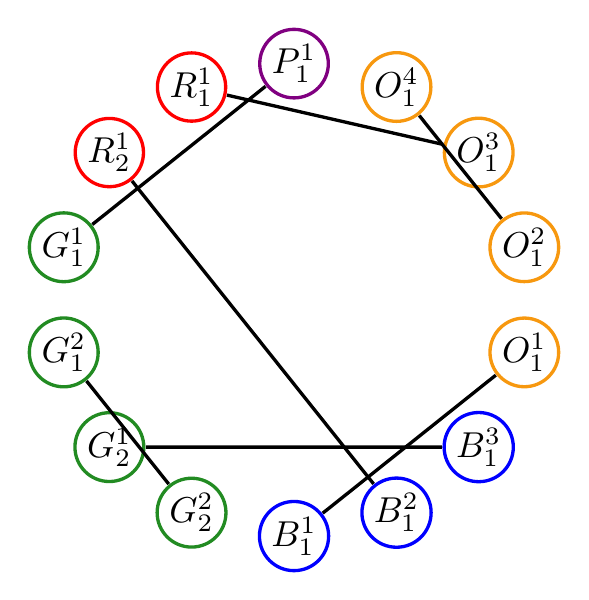
\begin{tikzpicture}[
mynode/.style={draw, circle, very thick, inner sep=1pt, scale=1.3},
myline/.style={draw, very thick},
]
\pgfmathsetmacro{\n}{14};
\pgfmathsetmacro{\r}{3};

\node[mynode,draw=Purple, circle] (1) at (0*360/\n + 90: \r cm)  {$\xcolor{P}_1^1$};
\node[mynode,draw=red] (2) at (1*360/\n + 90: \r cm)  {$\xcolor{R}_1^1$};
\node[mynode,draw=red] (3) at (2*360/\n + 90: \r cm)  {$\xcolor{R}_2^1$};
\node[mynode,draw=ForestGreen] (4) at (3*360/\n + 90: \r cm)  {$\xcolor{G}_1^1$};
\node[mynode,draw=ForestGreen] (5) at (4*360/\n + 90: \r cm)  {$\xcolor{G}_1^2$};
\node[mynode,draw=ForestGreen] (6) at (5*360/\n + 90: \r cm)  {$\xcolor{G}_2^1$};
\node[mynode,draw=ForestGreen] (7) at (6*360/\n + 90: \r cm)  {$\xcolor{G}_2^2$};
\node[mynode,draw=blue] (8) at (7*360/\n + 90: \r cm)  {$\xcolor{B}_1^1$};
\node[mynode,draw=blue] (9) at (8*360/\n + 90: \r cm)  {$\xcolor{B}_1^2$};
\node[mynode,draw=blue] (10) at (9*360/\n + 90: \r cm)  {$\xcolor{B}_1^3$};
\node[mynode,draw=YellowOrange] (11) at (10*360/\n + 90: \r cm)  {$\xcolor{O}_1^1$};
\node[mynode,draw=YellowOrange] (12) at (11*360/\n + 90: \r cm)  {$\xcolor{O}_1^2$};
\node[mynode,draw=YellowOrange] (13) at (12*360/\n + 90: \r cm)  {$\xcolor{O}_1^3$};
\node[mynode,draw=YellowOrange] (14) at (13*360/\n + 90: \r cm)  {$\xcolor{O}_1^4$};

\draw [myline] (14) -- (12);
\draw [myline] (13) -- (2);
\draw [myline] (11) -- (8);
\draw [myline] (10) -- (6);
\draw [myline] (9) -- (3);
\draw [myline] (7) -- (5);
\draw [myline] (4) -- (1);

\end{tikzpicture}
}
}
\caption{\mypm{}~115986.\label{fig:inter2_3}}
\end{subfigure}


\caption{Select interconnectivity graphs for Example 2.\label{fig:inter2}}

\end{figure}
